% -*- latex -*-
%%%%%%%%%%%%%%%%%%%%%%%%%%%%%%%%%%%%%%%%%%%%%%%%%%%%%%%%%%%%%%%%
%%%%%%%%%%%%%%%%%%%%%%%%%%%%%%%%%%%%%%%%%%%%%%%%%%%%%%%%%%%%%%%%
%%%%
%%%% This text file is part of the source of 
%%%% `Parallel Programming in MPI and OpenMP'
%%%% by Victor Eijkhout, copyright 2012-2021
%%%%
%%%% mpi-bcastreduce.tex : about broadcast & reduce collectives
%%%%
%%%%%%%%%%%%%%%%%%%%%%%%%%%%%%%%%%%%%%%%%%%%%%%%%%%%%%%%%%%%%%%%
%%%%%%%%%%%%%%%%%%%%%%%%%%%%%%%%%%%%%%%%%%%%%%%%%%%%%%%%%%%%%%%%

\Level 0 {Scan operations}
\label{sec:scan}

The \indexmpishow{MPI_Scan} operation also performs a reduction, but it keeps 
the partial results. That is, if processor~$i$ contains a number~$x_i$, 
and $\oplus$ is an operator,
then the scan operation leaves $x_0\oplus\cdots\oplus x_i$ on processor~$i$.
This type of operation is often called a \indexterm{prefix operation};
see \HPSCref{app:prefix}.

The \indexmpiref{MPI_Scan} routine is an \indextermsub{inclusive}{scan} operation,
meaning that it includes the data on the process itself;
\indexmpishow{MPI_Exscan} (see section~\ref{sec:mpi-exscan})
is exclusive, and does not include the data on the calling process.

\[
\begin{array}{rccccc}
  \mathrm{process:}
      &0&1&2&\cdots&p-1\\
  \mathrm{data:}
      &x_0&x_1&x_2&\cdots&x_{p-1}\\
  \mathrm{inclusive:}\mathstrut
      &x_0&x_0\oplus x_1&x_0\oplus x_1\oplus x_2&\cdots&\mathop\oplus_{i=0}^{p-1} x_i\\
  \mathrm{exclusive:}\mathstrut
      &\mathrm{unchanged}&x_0&x_0\oplus x_1&\cdots&\mathop\oplus_{i=0}^{p-2} x_i\\
\end{array}
\]

\cverbatimsnippet[examples/mpi/c/scan.c]{iscan}

In python native mode the result is a function return value,
with numpy the result is passed as the second parameter.
%
\pverbatimsnippet[examples/mpi/p/scan.py]{scanp}

You can use any of the given reduction operators,
  (for the list, see section~\ref{sec:operator-list}),
or a user-defined one. In the latter case,
the \indexmpishow{MPI_Op} operations do not return an error code.

\begin{mplnote}{Scan operations}
  As in the C/F interfaces, \ac{MPL} interfaces to the scan routines
  have the same calling sequences as the `Allreduce' routine.
\end{mplnote}

\Level 1 {Exclusive scan}
\label{sec:mpi-exscan}

Often, the more useful variant is the \indextermsub{exclusive}{scan}
%
\indexmpiref{MPI_Exscan}
%
with the same prototype. 

The result of the exclusive scan is undefined on processor~0
(\n{None} in python),
and on processor~1 it is a copy of the send value of processor~1.
In particular, the \indexmpishow{MPI_Op} need not be called on these two 
processors.

\begin{exercise}
  The exclusive definition, which computes $x_0\oplus x_{i-1}$ on
  processor~$i$, can easily be derived from the inclusive operation
  for operations such as \indexmpishow{MPI_SUM} or
  \indexmpishow{MPI_PROD}.  Are there operators where that is not the
  case?
\end{exercise}

\Level 1 {Use of scan operations}

The \indexmpishow{MPI_Scan} operation is often useful with indexing data. Suppose that
every processor~$p$ has a local vector where the number of elements~$n_p$ is dynamically 
determined. In order to translate the local numbering $0\ldots n_p-1$ to a global numbering
one does a scan with the number of local elements as input. The output is then the global 
number of the first local variable.

\begin{figure}[ht]
  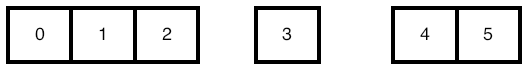
\includegraphics[scale=.5]{scanints}
  \caption{Local arrays that together form a consecutive range}
  \label{fig:scanints}
\end{figure}

\begin{exercise}
  \label{ex:scanprint}
  \begin{itemize}
  \item Let each process compute a random value $n_{\scriptstyle\mathrm{local}}$,
    and allocate an array of that length.
    Define \[ N=\sum n_{\scriptstyle\mathrm{local}} \]
  \item Fill the array with consecutive integers, so that all local arrays,
    laid end-to-end,
    contain the numbers~$0\cdots N-1$. (See figure~\ref{fig:scanints}.)
  \end{itemize}
  \skeleton{scangather}
\end{exercise}

\begin{exercise}
  Did you use \indexmpishow{MPI_Scan} or \indexmpishow{MPI_Exscan} for
  the previous exercise?
  How would you describe the result of the other scan operation, given the
  same input?
\end{exercise}

%% Exclusive scan examples:
%% %
%% \cverbatimsnippet[examples/mpi/c/exscan.c]{myfirst}
%% %
%% \pverbatimsnippet[examples/mpi/p/exscan.py]{exscanp}

It is possible to do a \indexterm{segmented scan}. Let $x_i$ be a series of numbers
that we want to sum to $X_i$ as follows. Let $y_i$ be a series of booleans such that
\[ 
\begin{cases}
  X_i=x_i&\hbox{if $y_i=0$}\\
  X_i=X_{i-1}+x_i&\hbox{if $y_i=1$}
\end{cases}
\]
(This is the basis for the implementation of the \indexterm{sparse matrix vector product}
as prefix operation; see \HPSCref{sec:spmvp-prefix}.)
This means that $X_i$ sums the segments between locations where $y_i=0$ and the
first subsequent place where $y_i=1$. To implement this, you need a user-defined operator
\[ 
\begin{pmatrix}  X\\ x\\ y\end{pmatrix}
=
\begin{pmatrix}  X_1\\ x_1\\ y_1\end{pmatrix}
\bigoplus
\begin{pmatrix}  X_2\\ x_2\\ y_2\end{pmatrix}\colon
  \begin{cases}
    X=x_1+x_2&\hbox{if $y_2==1$}\\ X=x_2&\hbox{if $y_2==0$}
  \end{cases}
\]
This operator is not communitative, and it needs to be declared as such
with \indexmpishow{MPI_Op_create}; see section~\ref{sec:mpi-op-create}


